\PassOptionsToPackage{numbers,sort&compress}{natbib}
\documentclass[11pt,logo,nonumbering]{preprint}
\usepackage{amsmath,amssymb,mathtools,booktabs,tabularx,array,microtype}
\usepackage{natbib}
\usepackage{xcolor,tikz,fancyhdr,placeins,pgfplots,multirow}
\pgfplotsset{compat=1.18}
\captionsetup{font=small,labelfont=bf}
\usepackage[colorlinks=true,linkcolor=blue!45!black,citecolor=blue!45!black,urlcolor=blue!55!black]{hyperref}
\usetikzlibrary{arrows.meta,positioning,fit,shapes.geometric}
\setlength{\parindent}{0pt}
\setlength{\emergencystretch}{2em}
\definecolor{primaryblue}{RGB}{0,51,102}
\definecolor{lightblue}{RGB}{220,235,252}
\definecolor{sciencegreen}{RGB}{0,168,150}
\definecolor{darkgreen}{RGB}{0,128,96}
\definecolor{cautionorange}{RGB}{210,112,45}
\hypersetup{pdftitle={Maturation-Aware Drug Prioritization for Acute Myeloid Leukemia},
 pdfauthor={Vania Halim},pdfsubject={Computational medicine project report}}
\newcommand{\z}{z}
\newcommand{\pk}{\text{prec@5}}
\newcolumntype{Y}{>{\raggedright\arraybackslash}X}
\title{Maturation-Aware Drug Prioritization for Acute Myeloid Leukemia}
\author{
  \textit{Predicting the ex vivo drug screen from molecular profiles, and testing its clinical relevance}\\[0.8em]
  % TODO: add teammates' names and Andrew IDs
  \textbf{Vania Halim}\quad\textbf{[Teammate 2]}\quad\textbf{[Teammate 3]}\\
  Carnegie Mellon University\\
  \texttt{vphalim@andrew.cmu.edu}\\[0.5em]
  {\small Computational Medicine project report}
}
\date{November 2026}
\begin{document}
\maketitle
\begin{abstract}
Ex vivo drug screens can show which drugs kill a patient's leukemia cells, but they need fresh cells, take days to weeks and run at few centers, whereas sequencing is routine. We ask whether a patient's molecular profile at diagnosis can rank the drugs on the Beat AML screen in the order the screen itself would, and whether that ranking carries clinical information. The target is drug-standardized AUC, so that a ranking must find patient-specific sensitivity rather than reproduce general drug potency. A per-drug ridge model on mutations, fusions, clinical variables and the interpretable expression features of \citet{bottomly2022} (six cell-type maturation scores, nine co-expression modules, PEAR1 and LSC17) was selected by cross-validation in Waves1+2 (266 patients, 116 drugs) and scored once on Waves3+4 (163 patients). On the holdout, 46\% of its top-5 recommendations were drugs the patient was truly sensitive to, against 38\% for genotype-matched rules and 25\% by chance (paired gain $+0.074$, 95\% CI $[0.034, 0.117]$). Most of the gain comes from the maturation scores, and it is concentrated in patients without an actionable mutation, for whom the rules do no better than chance. Venetoclax response was predicted with Spearman $\rho=0.77$. The clinical arm was negative. Observed ex vivo cytarabine sensitivity did not predict response to induction chemotherapy (odds ratio $1.02$ per SD, $p=0.94$, 145 patients), and neither did the predicted value. The predicted score was associated with overall survival after adjustment for ELN2017 risk and age in Beat AML (hazard ratio $1.33$ per SD, $p=0.005$), but this did not replicate in TCGA-LAML (HR $0.94$, $[0.74, 1.19]$). Molecular profiles can stand in for the ex vivo screen as a drug-ranking tool; we found no evidence that either the screen or our predictions of it, for cytarabine, anticipate clinical response.
\end{abstract}

\section{Introduction and motivation}
Acute myeloid leukemia (AML) is treated mostly by risk group. Fit patients receive intensive induction (``7+3'' cytarabine and an anthracycline), unfit patients receive venetoclax with a hypomethylating agent \citep{dinardo2020viale}, and targeted inhibitors are added when the tumor carries an actionable lesion such as FLT3-ITD or an IDH mutation \citep{dohner2017eln}. Many patients have no actionable lesion, and response within a risk group varies widely.

Functional precision medicine tests drugs directly on a patient's cells. Small prospective studies report clinical benefit when treatment follows such screens \citep{kornauth2022,malani2022}. The Beat AML programme screened about 120 drugs on primary AML samples alongside exome and RNA sequencing \citep{tyner2018,bottomly2022}. \citet{bottomly2022} found that drug response depends on the tumor's maturation state, captured by six cell-type scores derived from single-cell data \citep{vangalen2019}: venetoclax works on progenitor-like tumors and fails on monocytic ones, and MEK inhibitors show the reverse. They also found that mutation effects on drug response depend on cell type. They used these results descriptively and did not build a predictor.

\textbf{The task.} For each patient, rank the drugs on the panel from most to least likely to be effective, using only data available at diagnosis: mutations, fusions, clinical variables and bulk RNA-seq. A good ranking places drugs the patient's cells were truly sensitive to near the top.

\textbf{Hypotheses.} (H1) A learned model beats clinician-style genotype-matched rules at the top of the ranking, on patients not used for any modelling choice. (H2) Maturation features add to genomics. (H3) The predicted sensitivity to cytarabine, the backbone of induction, relates to induction response and survival.

\section{Related work and background}
\textbf{Ex vivo screens in AML.} Beat AML released drug response, exome and RNA-seq data for several hundred patients \citep{tyner2018} and extended them in a second release with clinical follow-up \citep{bottomly2022}. That study introduced the maturation-state view of drug response, the nine non-redundant co-expression modules computed with WGCNA \citep{langfelder2008wgcna}, and PEAR1 expression as a prognostic marker. The LSC17 stemness score is an independent 17-gene prognostic signature \citep{ng2016lsc17}.

\textbf{Functional precision medicine.} Prospective studies that treat patients according to their ex vivo screens report response in a subset \citep{kornauth2022,malani2022}. Those studies require the screen itself. Our question is whether the screen's information can be recovered from molecular data alone, which would make it available to every patient.

\textbf{What is different here.} Most drug-response prediction work reports per-drug correlation across patients. A clinician needs the reverse: an ordering of drugs \emph{within one patient}. We therefore grade within-patient rankings against a drug-standardized target, compare against an explicit genomic-rule baseline, and test the predictions against clinical endpoints that are never used in training.

\section{Methodology}
\subsection{Data and cohorts}
We use the Beat AML waves 1--4 release \citep{bottomly2022}. The modelling cohort is the 429 patients with both RNA-seq and a drug screen, one specimen of each per patient. Following the paper, Waves1+2 (266 patients) are the training cohort and Waves3+4 (163 patients, accrued later) are the test cohort. We keep the 116 drugs tested on at least 60 Waves1+2 patients; this choice uses only how many patients were tested, not their results. The patient-by-drug matrix is 28\% missing (35{,}932 tested pairs; median 92 drugs per patient), and each patient is graded only on drugs tested on their cells. Figure~\ref{fig:design} shows how the cohorts are used.

\begin{figure}[ht]
\centering
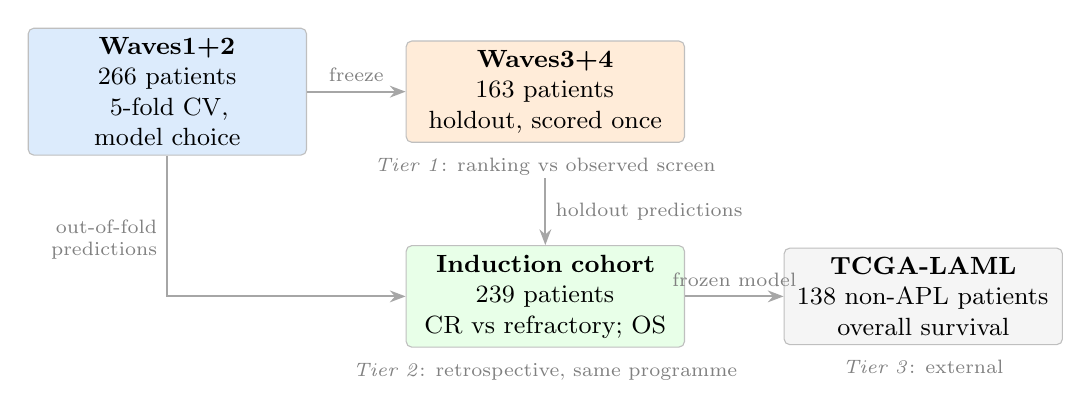
\begin{tikzpicture}[
 box/.style={draw=gray!50,rounded corners=2pt,minimum height=1.15cm,font=\small,align=center,text width=3.3cm},
 train/.style={box,fill=lightblue},
 test/.style={box,fill=orange!15},
 clin/.style={box,fill=green!9},
 ext/.style={box,fill=gray!8},
 tier/.style={font=\scriptsize,gray,align=center},
 arr/.style={-{Stealth[length=2mm]},gray!70,thick}]
 \node[train] (cv) at (0,0) {\textbf{Waves1+2}\\266 patients\\5-fold CV, model choice};
 \node[test]  (ho) at (4.8,0) {\textbf{Waves3+4}\\163 patients\\holdout, scored once};
 \node[clin]  (cl) at (4.8,-2.6) {\textbf{Induction cohort}\\239 patients\\CR vs refractory; OS};
 \node[ext]   (tc) at (9.6,-2.6) {\textbf{TCGA-LAML}\\138 non-APL patients\\overall survival};
 \node[tier,below=2pt of ho] {\textit{Tier 1}: ranking vs observed screen};
 \node[tier,below=2pt of cl] {\textit{Tier 2}: retrospective, same programme};
 \node[tier,below=2pt of tc] {\textit{Tier 3}: external};
 \draw[arr] (cv) -- node[above,font=\scriptsize,gray]{freeze} (ho);
 \draw[arr] (cv.south) |- node[pos=0.3,left,font=\scriptsize,gray,align=right]{out-of-fold\\predictions} (cl.west);
 \draw[arr] (ho.south) ++(0,-0.45) -- node[right,font=\scriptsize,gray]{holdout predictions} (cl.north);
 \draw[arr] (cl) -- node[above,font=\scriptsize,gray]{frozen model} (tc);
\end{tikzpicture}
\caption{Study design. All modelling choices were made by cross-validation within Waves1+2. The frozen model was then scored once on Waves3+4 (ranking validation), related to induction response and survival using predictions that are out-of-sample for every patient, and applied unchanged to TCGA-LAML.}
\label{fig:design}
\end{figure}


\subsection{Target}
Raw AUC mixes drug potency (some drugs kill nearly every sample at the tested doses), the patient's general sensitivity, and patient-specific response. Ranking by raw AUC mostly reproduces potency, which is the same for every patient. The target is therefore the drug-standardized AUC,
\begin{equation}
 \z_{pd}=\frac{\mathrm{AUC}_{pd}-\mu_d}{\sigma_d},
\end{equation}
with $\mu_d,\sigma_d$ estimated on training patients only. $\z<0$ means the patient's cells are more sensitive to drug $d$ than a typical AML sample. A patient counts as \emph{truly sensitive} when $\z<-0.84$, the 20th percentile of a standard normal; the observed share is 17.8\% in Waves1+2. This cutoff is our choice; threshold-free metrics are reported alongside.

\subsection{Features}
All features are interpretable and come from \citet{bottomly2022}: six van Galen cell-type scores \citep{vangalen2019} (HSC-, progenitor-, GMP-, promonocyte-, monocyte- and cDC-like), nine WGCNA module eigengenes, PEAR1 expression and the LSC17 score; 20 mutations and 4 fusions carried by at least 10 training patients; and age, de novo status and specimen tissue (44 features). Cell-type scores and module eigengenes are first principal components of fixed gene sets, fitted on the 372 Waves1+2 RNA-seq specimens. They reproduce the published scores exactly ($r=1.0$), and contain no Waves3+4 patient. Patients without DNA sequencing (17 training, 2 test) receive zeros for mutations plus a missing-DNA indicator.

\subsection{Models}
Every model outputs a score per (patient, drug); lower means recommend first.
\begin{enumerate}
 \item \textbf{Random} and \textbf{B0 population}: a random order, and one list for everyone ordered by mean training AUC.
 \item \textbf{B1 genomic rules}: drugs whose curated targets match one of the patient's alterations come first (FLT3/FLT3-ITD $\rightarrow$ FLT3 inhibitors, NRAS/KRAS/PTPN11 $\rightarrow$ MEK inhibitors, KIT, JAK2, BCR-ABL1, IDH1/2), then B0's order. Targets come from the paper's curated drug--gene table. This is the clinician-style bar to beat.
 \item \textbf{M1 per-drug ridge}: one ridge regression per drug predicting $\z$ from standardized features, with the penalty chosen by efficient leave-one-out over 21 values \citep{pedregosa2011sklearn}.
 \item \textbf{M2 pooled gradient boosting}: one XGBoost model \citep{chen2016xgboost} over all (patient, drug) pairs, with drug identity, kinase-family membership and a ``drug targets one of this patient's mutated genes'' indicator, so that information is shared across drugs (depth 4, 400 trees, learning rate 0.05, fixed in advance).
\end{enumerate}
Ablations fit M1 on mutations + clinical only, adding cell-type scores, expression only, and all features. Hybrids place B1's rule matches on top of M1 or M2. A shuffled-label M1, which permutes each drug's targets across patients, measures the pipeline's chance level.

\subsection{Evaluation}
Metrics are computed per patient over that patient's tested drugs and then averaged, with 95\% patient-bootstrap intervals (1{,}000 resamples). \textbf{Precision@5} is the fraction of the top five recommended drugs that are truly sensitive. Its chance value is the patient's \emph{prevalence} of sensitive drugs, and \textbf{lift@5} is precision@5 minus prevalence. We also report NDCG@10 with gain $\max(0,-\z)$ and the Spearman correlation between score and $\z$. Model comparisons use paired bootstrap differences on the same patients. All choices were made by 5-fold cross-validation within Waves1+2, refitting the $\z$-scaling and every model inside each fold. The model list was then frozen and Waves3+4 scored once.

\subsection{Clinical validation}
\textbf{Induction response.} Patients sampled at initial diagnosis who received standard-chemotherapy induction with a recorded outcome form the clinical cohort: 239 patients, 74 refractory and 165 with complete response (CR or CRi). A stricter subset with 7+3 or HiDAC recorded has 175 patients (45 refractory). The predicted cytarabine $\z$ is out-of-sample for every patient: out-of-fold predictions for Waves1+2 and holdout predictions for Waves3+4. Outcome labels are never used in training. We fit logistic regressions of refractory status on ELN2017 risk group and age, adding the observed or predicted cytarabine $\z$, and report odds ratios per SD, likelihood-ratio tests and 20-times-repeated 5-fold cross-validated AUROC.

\textbf{Survival.} Cox models of overall survival on the predicted score, ELN2017 and age \citep{davidson2019lifelines}.

\textbf{External survival validation.} TCGA-LAML \citep{tcga2013laml} was obtained from cBioPortal \citep{cerami2012cbioportal}: PanCanAtlas RNA-seq, exome mutation calls and overall survival, with age and karyotype from the 2013 study. The frozen M1 model, fit on Waves1+2 exactly as for the holdout, was applied without refitting. Because the expression platform differs, cell-type and module scores are computed by z-scoring TCGA genes within TCGA and projecting them on the PC1 loadings learned in Beat AML, and every expression feature is then rescaled to the Beat AML training distribution. FLT3-ITD is called from in-frame insertions at codons 560--620, and fusions from karyotype. ELN2017 is approximated from karyotype and mutations, without FLT3-ITD allelic ratio. Acute promyelocytic leukemia (APL), which is treated differently, is excluded from the primary analysis. The pre-specified test is the hazard ratio of the predicted score adjusted for approximate ELN and age.

\section{Experiments}
\subsection{Software verification}
Fifteen automated tests pass. They check that the computed cell-type scores reproduce the published values; that no Waves3+4 patient enters any fit during cross-validation; that training-patient features do not change when test expression is scrambled; that the $\z$-scaler and both learned models give identical held-out predictions when held-out AUCs are altered; and that the shuffled-label model is at chance. The full experiment regenerates from the raw data with \texttt{python -m src.run\_models [-{}-holdout]}, \texttt{python -m src.clinical} and \texttt{python -m src.tcga}.

\subsection{Recommendation performance}
Table~\ref{tab:main} and Figure~\ref{fig:main} give the results. In cross-validation, M1 with all features is the best model. 33\% of its top five recommendations are truly sensitive, against 25\% for B1 and 18\% by chance, a paired gain over B1 of $+0.076$ $[0.050, 0.104]$. On the holdout, scored once, the gain replicates almost exactly ($+0.074$ $[0.034, 0.117]$). M1 also ranks the whole list far better than B1 (Spearman $0.27$ vs $0.07$ on the holdout). B1 by design reorders only a handful of drugs.

\begin{table}[ht]
\small
\centering
\caption{Per-patient ranking metrics, mean over patients (95\% patient-bootstrap CI for precision@5). CV: 5-fold within Waves1+2, 262 patients with at least 10 tested drugs. Holdout: fit on Waves1+2, scored once on Waves3+4, 151 patients. $\Delta$: paired difference in precision@5 against B1. Chance (prevalence) is 0.180 in CV and 0.253 on the holdout.}
\label{tab:main}
\setlength{\tabcolsep}{4pt}
\begin{tabular}{@{}lcccccc@{}}
\toprule
 & \multicolumn{3}{c}{Cross-validation} & \multicolumn{3}{c}{Holdout (Waves3+4)}\\
\cmidrule(lr){2-4}\cmidrule(l){5-7}
Model & Prec@5 & NDCG@10 & $\Delta$ vs B1 & Prec@5 & NDCG@10 & $\Delta$ vs B1\\
\midrule
Random & 0.179 & 0.225 & $-0.073$ & 0.234 & 0.233 & $-0.147$\\
B0 population & 0.188 & 0.245 & $-0.064$ & 0.318 & 0.293 & $-0.064$\\
B1 genomic rules & 0.252 & 0.295 & -- & 0.381 & 0.343 & --\\
M1 ridge, mutations + clin. & 0.289 & 0.335 & $+0.037$ & 0.409 & 0.363 & $+0.028$\\
M1 ridge, + cell types & 0.320 & 0.382 & $+0.068$ & \textbf{0.464} & 0.417 & $+0.082$\\
M1 ridge, expression only & 0.293 & 0.364 & $+0.041$ & 0.428 & 0.389 & $+0.046$\\
M1 ridge, all features & \textbf{0.328} & \textbf{0.393} & $+0.076$ & 0.456 & \textbf{0.422} & $+0.074$\\
M2 XGBoost, mutations + clin. & 0.295 & 0.334 & $+0.043$ & 0.367 & 0.344 & $-0.015$\\
M2 XGBoost, all features & 0.299 & 0.366 & $+0.047$ & 0.430 & 0.383 & $+0.049$\\
B1 rules, then M1 all & 0.321 & 0.382 & $+0.069$ & 0.440 & 0.403 & $+0.058$\\
M1, shuffled labels & 0.195 & 0.230 & $-0.056$ & 0.257 & 0.235 & $-0.125$\\
\midrule
\multicolumn{7}{@{}p{0.95\textwidth}@{}}{\footnotesize 95\% CI of $\Delta$ for M1 all: CV $[+0.050, +0.104]$, holdout $[+0.034, +0.117]$; for M1 + cell types: $[+0.039, +0.098]$ and $[+0.044, +0.121]$.}\\
\bottomrule
\end{tabular}
\end{table}

\begin{figure}[ht]
\centering
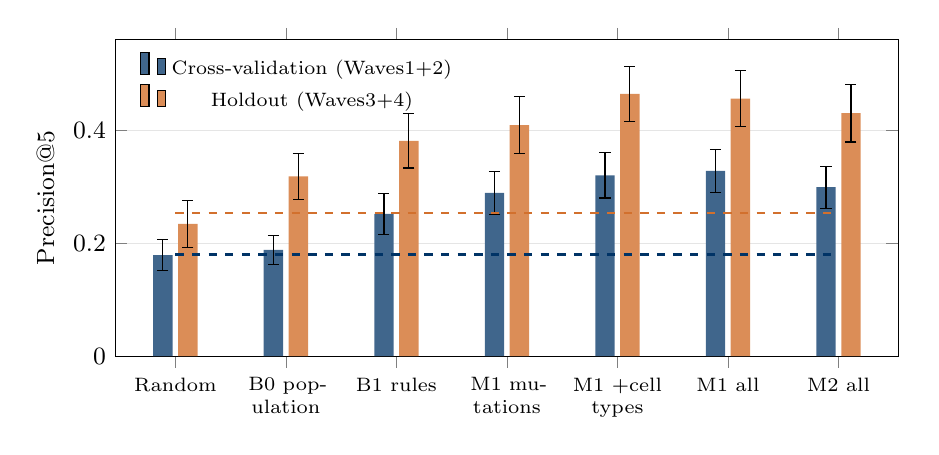
\begin{tikzpicture}
\begin{axis}[
  ybar, bar width=7pt, width=0.95\textwidth, height=5.6cm,
  symbolic x coords={Random,B0,B1,M1mut,M1ct,M1all,M2all},
  xticklabels={Random,B0 population,B1 rules,{M1 mutations},{M1 +cell types},{M1 all},{M2 all}},
  xtick=data, x tick label style={font=\scriptsize,align=center,text width=1.6cm},
  ylabel={Precision@5}, ymin=0, ymax=0.56,
  yticklabel style={/pgf/number format/fixed,/pgf/number format/precision=2},
  legend style={font=\scriptsize,at={(0.02,0.98)},anchor=north west,draw=none,fill=none},
  tick label style={font=\small}, label style={font=\small},
  ymajorgrids, grid style={gray!20}, enlarge x limits=0.09,
  error bars/y dir=both, error bars/y explicit]
\addplot[fill=primaryblue!75,draw=none] coordinates {
 (Random,0.179) +- (0,0.028) (B0,0.188) +- (0,0.026) (B1,0.252) +- (0,0.036) (M1mut,0.289) +- (0,0.038)
 (M1ct,0.320) +- (0,0.040) (M1all,0.328) +- (0,0.038) (M2all,0.299) +- (0,0.037)};
\addlegendentry{Cross-validation (Waves1+2)}
\addplot[fill=cautionorange!80,draw=none] coordinates {
 (Random,0.234) +- (0,0.042) (B0,0.318) +- (0,0.040) (B1,0.381) +- (0,0.048) (M1mut,0.409) +- (0,0.051)
 (M1ct,0.464) +- (0,0.049) (M1all,0.456) +- (0,0.050) (M2all,0.430) +- (0,0.051)};
\addlegendentry{Holdout (Waves3+4)}
\draw[primaryblue,dashed,thick] (axis cs:Random,0.180) -- (axis cs:M2all,0.180);
\draw[cautionorange,dashed,thick] (axis cs:Random,0.253) -- (axis cs:M2all,0.253);
\end{axis}
\end{tikzpicture}
\caption{Precision@5 with 95\% patient-bootstrap intervals (approximately symmetric half-widths shown). Dashed lines: chance (mean prevalence of truly sensitive drugs) in each cohort. Holdout values are higher for every model because Waves3+4 samples are more drug-sensitive overall (Section~\ref{sec:analysis}); compare models within a cohort.}
\label{fig:main}
\end{figure}

\subsection{Ablation: maturation state adds to genomics}
With mutations and clinical variables alone, M1 already beats the hand-written rules slightly ($+0.037$ in CV; $+0.028$, CI including zero, on the holdout). Adding the six cell-type scores is the largest single improvement: lift@5 rises from $0.108$ to $0.139$ in CV and from $0.156$ to $0.210$ on the holdout. Modules, PEAR1 and LSC17 add little on top. Expression alone performs about as well as genomics alone, and the two are complementary. This is the predictive counterpart of the descriptive finding of \citet{bottomly2022}: maturation state carries drug-response information that genomics does not.

\subsection{Who benefits}
Table~\ref{tab:subgroups} splits patients by actionable lesion. For the 94 training and 50 holdout patients with no lesion that B1 has a rule for, B1 falls back to the population list and does no better than chance. M1 doubles precision@5 in CV ($0.245$ vs $0.123$, chance $0.153$) and improves it on the holdout ($0.416$ vs $0.300$, chance $0.260$). For FLT3-ITD patients, where the rules work well, M1 matches or slightly exceeds them. This group also contains the few patients without DNA sequencing.

\begin{table}[ht]
\small
\centering
\caption{Precision@5 by genomic subgroup. ``Random'' is each group's chance level. RAS pathway: NRAS, KRAS or PTPN11 mutation.}
\label{tab:subgroups}
\begin{tabular}{@{}lcccccccc@{}}
\toprule
 & \multicolumn{4}{c}{Cross-validation} & \multicolumn{4}{c}{Holdout}\\
\cmidrule(lr){2-5}\cmidrule(l){6-9}
Subgroup & $n$ & Random & B1 & M1 all & $n$ & Random & B1 & M1 all\\
\midrule
FLT3-ITD & 60 & 0.283 & 0.497 & \textbf{0.557} & 38 & 0.289 & 0.426 & \textbf{0.516}\\
RAS pathway & 62 & 0.129 & 0.265 & \textbf{0.332} & 41 & 0.161 & 0.444 & \textbf{0.522}\\
No actionable lesion & 94 & 0.153 & 0.123 & \textbf{0.245} & 50 & 0.260 & 0.300 & \textbf{0.416}\\
\bottomrule
\end{tabular}
\end{table}

\subsection{Which drugs are predictable}
Across all 116 drugs, the median Spearman correlation between predicted and observed $\z$ across held-out patients is $0.31$ (CV) and $0.30$ (holdout) for M1 with all features, against $0.20$ for mutations alone and $0.00$ for shuffled labels. Table~\ref{tab:drugs} shows clinically relevant drugs. Venetoclax is the clearest case. Its predictability rises from $0.43$ to $0.77$ on the holdout once expression is added, reflecting the progenitor-versus-monocytic biology described by \citet{bottomly2022}. MEK inhibitors also gain substantially from expression. FLT3 inhibitors are largely predictable from mutations alone. Cytarabine is moderate ($0.31$ on the holdout), and azacytidine is barely predictable.

\begin{table}[ht]
\small
\centering
\caption{Per-drug Spearman correlation between predicted and observed $\z$ across held-out patients, for M1 with mutations + clinical (``Mut.'') and with all features (``All''). $n$: holdout patients tested.}
\label{tab:drugs}
\begin{tabular}{@{}llccccc@{}}
\toprule
 & & \multicolumn{2}{c}{Cross-validation} & \multicolumn{3}{c}{Holdout}\\
\cmidrule(lr){3-4}\cmidrule(l){5-7}
Drug & Class & Mut. & All & $n$ & Mut. & All\\
\midrule
Venetoclax & BCL2 & 0.20 & 0.65 & 138 & 0.43 & \textbf{0.77}\\
Cytarabine & chemotherapy & 0.35 & 0.45 & 135 & 0.21 & 0.31\\
Azacytidine & hypomethylating & 0.05 & 0.13 & 94 & 0.04 & 0.20\\
Sorafenib & FLT3 (multi-kinase) & 0.49 & 0.57 & 146 & 0.46 & 0.52\\
Quizartinib & FLT3 & 0.47 & 0.48 & 133 & 0.27 & 0.30\\
Gilteritinib & FLT3 & 0.12 & 0.21 & 110 & 0.15 & 0.23\\
Midostaurin & FLT3 (multi-kinase) & 0.50 & 0.50 & 107 & 0.37 & 0.44\\
Crenolanib & FLT3 & 0.47 & 0.59 & 96 & 0.53 & 0.60\\
Trametinib & MEK & 0.33 & 0.57 & 142 & 0.30 & 0.58\\
Selumetinib & MEK & 0.22 & 0.54 & 114 & 0.47 & 0.64\\
\bottomrule
\end{tabular}
\end{table}

\subsection{Clinical validation: induction response}
Table~\ref{tab:clinical} gives the induction results. The \emph{observed} ex vivo cytarabine $\z$, available for the 145 clinical-cohort patients whose cells were tested with cytarabine, does not separate refractory from responding patients (univariate AUROC $0.49$; adjusted odds ratio $1.02$ per SD, $p=0.94$). The \emph{predicted} $\z$ does not improve on ELN2017 and age either (cross-validated AUROC $0.736$ vs $0.739$). In the 7+3/HiDAC subset it reaches borderline significance ($p=0.049$), but in the unexpected direction: patients predicted to be more cytarabine-resistant were \emph{less} often refractory. We treat this as noise. PEAR1 and LSC17 did not add to ELN and age here either.

\begin{table}[ht]
\small
\centering
\caption{Refractory vs complete response after standard-chemotherapy induction. OR per SD of the added term, adjusted for ELN2017 and age. AUROC: 20$\times$ repeated 5-fold cross-validation. $p$: likelihood-ratio test against ELN + age. The observed-$\z$ row is fitted on the 145 patients tested with cytarabine, so its AUROC is not directly comparable.}
\label{tab:clinical}
\setlength{\tabcolsep}{4pt}
\begin{tabular}{@{}llcccc@{}}
\toprule
Cohort & Model & $n$ (refractory) & OR per SD [95\% CI] & CV AUROC & $p$\\
\midrule
\multirow{4}{*}{All standard chemo} & ELN + age & 238 (74) & -- & 0.739 & --\\
 & + observed cytarabine $\z$ & 145 (40) & 1.02 [0.67, 1.54] & 0.707 & 0.94\\
 & + predicted cytarabine $\z$ & 238 (74) & 0.78 [0.57, 1.07] & 0.736 & 0.13\\
 & + PEAR1 + LSC17 & 238 (74) & -- & 0.733 & 0.23\\
\midrule
\multirow{3}{*}{7+3 / HiDAC} & ELN + age & 175 (45) & -- & 0.719 & --\\
 & + observed cytarabine $\z$ & 110 (30) & 1.17 [0.71, 1.92] & 0.733 & 0.53\\
 & + predicted cytarabine $\z$ & 175 (45) & 0.68 [0.46, 1.01] & 0.738 & 0.049\\
\bottomrule
\end{tabular}
\end{table}

\subsection{Clinical validation: survival and external replication}
In Beat AML, a higher predicted cytarabine-resistance score was associated with shorter overall survival: hazard ratio $1.50$ per SD alone ($[1.22, 1.85]$, $p<0.001$) and $1.33$ ($[1.09, 1.62]$, $p=0.005$) after adjustment for ELN2017 and age (229 patients, 100 deaths; C-index $0.744\rightarrow0.754$). The observed score showed no association ($0.91$, $[0.72, 1.15]$, $p=0.43$; 142 patients). The association was unchanged after adjustment for de novo status ($1.32$) and similar in de novo patients only ($1.28$, $[1.00, 1.65]$, $p=0.052$).

This association was the pre-specified target for external validation, and it \textbf{did not replicate} (Table~\ref{tab:tcga}). In TCGA-LAML, the adjusted hazard ratio was $0.94$ ($[0.74, 1.19]$, $p=0.59$; 138 non-APL patients, 91 deaths), and the predicted score did not improve on approximate ELN and age (C-index $0.640$ vs $0.638$). Including APL patients did not change this.

\begin{table}[ht]
\small
\centering
\caption{Overall survival: hazard ratio per SD of the predicted cytarabine $\z$ (higher = predicted more resistant), from the frozen M1 model. TCGA uses an approximate ELN2017 (karyotype + mutations).}
\label{tab:tcga}
\begin{tabular}{@{}llcccc@{}}
\toprule
Cohort & Adjustment & Patients (deaths) & HR per SD [95\% CI] & $p$ & C-index\\
\midrule
Beat AML & none & 229 (100) & 1.50 [1.22, 1.85] & $<0.001$ & 0.611\\
Beat AML & ELN + age & 229 (100) & 1.33 [1.09, 1.62] & 0.005 & 0.754\\
TCGA-LAML, non-APL & none & 138 (91) & 1.04 [0.83, 1.31] & 0.74 & 0.508\\
TCGA-LAML, non-APL & ELN + age & 138 (91) & 0.94 [0.74, 1.19] & 0.59 & 0.640\\
TCGA-LAML, all & ELN + age & 151 (94) & 0.88 [0.70, 1.11] & 0.27 & 0.663\\
\bottomrule
\end{tabular}
\end{table}

\section{Analysis}
\label{sec:analysis}
\textbf{Why the learned model beats the rules.} The rules encode one lesion--drug link each and leave the rest of the list in potency order, which for the drug-standardized target is no better than chance. The ridge model learns graded effects for every drug, including links no rule covers, and above all the dependence on maturation state. The ablation shows that most of the gain beyond genomics comes from six cell-type scores. These are cheap to compute from routine RNA-seq and have a direct biological reading.

\textbf{Pooling across drugs did not help.} M2 was designed to share information across drugs, which should help with only about 270 training patients. It was nonetheless worse than per-drug ridge, and with mutations only it failed to beat the rules on the holdout. With this many patients, a regularized linear model per drug was the better choice. Adding the rules on top of M1 did not help either, because M1 already learns the FLT3 links.

\textbf{The holdout cohort is more drug-sensitive.} 25.3\% of tested Waves3+4 pairs fall below the sensitivity cutoff, against 17.8\% in Waves1+2, using Waves1+2 scaling. Every model's holdout precision is higher as a result, and even the population list (B0) gains some lift on the holdout ($+0.064$). Likely causes are drift in the assay or sample processing between waves. Comparisons between models within the holdout, which are paired on the same patients, are unaffected, and they agree with cross-validation.

\textbf{Why the induction result is negative.} The predicted cytarabine score cannot be expected to anticipate induction response if the observed ex vivo result does not, and in this cohort it does not. Plausible reasons are that induction combines cytarabine with an anthracycline, which is not on the panel; that a short culture misses the marrow microenvironment and drug pharmacokinetics; and that induction failure partly reflects patient fitness. This is a finding about the ex vivo readout for cytarabine, not about the model.

\textbf{Why the survival result did not replicate.} Three explanations are possible and cannot be separated here. First, the Beat AML association may be a chance finding among the several clinical tests we ran. Second, TCGA's exome calls under-detect two of the cytarabine model's strongest inputs: FLT3-ITD, its largest weight, is called in 16\% of TCGA patients against 24\% in Beat AML, and SRSF2 in 2\% against 12\%. Third, the cohorts differ in era (TCGA patients were diagnosed 2001--2010), treatment and composition. The feature mapping itself appears sound. The mapped monocyte-like score separates FAB M4/M5 cases strongly (mean $3.6$ vs $-1.6$), predicted scores have a similar spread in both cohorts (SD $0.31$ vs $0.40$), and approximate ELN and age give a sensible C-index. A first TCGA run contained a bug: genes with missing values in the TCGA expression file made seven expression features undefined, and these were silently imputed. It was found by checking feature distributions and fixed before the results were interpreted, and the conclusion did not change.

\section{Limitations}
\begin{itemize}[leftmargin=1.5em,itemsep=2pt]
\item The ranking validation is internal. Waves3+4 are new patients, but from the same programme, assay and pipeline. An external cohort with both a drug screen and RNA-seq would be needed to validate the ranking itself.
\item The target is ex vivo sensitivity. A high-ranked drug is one the patient's cells respond to in culture; we show no evidence that treating by this ranking improves outcomes, and for cytarabine the ex vivo readout did not track induction response.
\item The sensitivity cutoff ($\z<-0.84$) is our choice, and the holdout's higher sensitivity rate shows that $\z$-scaling across waves is imperfect.
\item The clinical analyses are retrospective. Treatment was not assigned by the model, few patients received venetoclax-based induction, and anthracyclines are absent from the panel.
\item The TCGA analysis approximates ELN2017, lacks treatment details, and depends on exome mutation calls that miss some lesions.
\item Expression features were fitted on all Waves1+2 RNA-seq specimens, including patients held out within cross-validation folds. This uses no drug or outcome labels and does not affect the Waves3+4 holdout.
\end{itemize}

\section{Conclusion and future work}
Molecular profiles at diagnosis, and in particular the tumor's maturation state, recover a substantial part of the patient-specific information in the Beat AML ex vivo drug screen. A simple per-drug ridge model beats genotype-matched rules on patients accrued later, with the largest benefit for patients who have no actionable mutation. Venetoclax response is especially well predicted. We found no evidence that ex vivo cytarabine sensitivity, measured or predicted, anticipates response to induction, and an apparent survival association did not replicate externally. The most useful next steps are external validation of the ranking in a cohort with both screen and RNA-seq data, and a venetoclax-focused analysis comparing predicted sensitivity with outcomes of venetoclax-treated patients.

\FloatBarrier
\renewcommand{\bibsection}{\section*{References}}
\begingroup
\raggedright
\bibliographystyle{unsrtnat}
\bibliography{references}
\endgroup
\end{document}
